\chapter{Inledning}

En drönare är ett obemannat luftfordon \citep{geospatial}. För att drönare är mer versatila än robotar som inte flyger så finns det särskilda användningsfall för dem. De kan övervaka markföroreningar eller växternas behov av vatten och näring samt förhindra industriolyckor \citep{crowdsurveillance}. Drönare har också använts vid katastrofområden, som vid jordbävningen nära Japan för att mäta strålningsvärden i Fukushima och att skaffa visuell information om katastrofområdet samt i räddning av invandrare vid medelhavet. Inom logistikbranschen är man intresserad om autonoma drönaren som skulle leverera paket för kunder, till exempel 86 \% av Amazons paket väger mindre än 2.26 kg och de har tänkt på att leverera paket inom 30 minuter för människor som bor nära Amazons lager \citep{cbsnews}.

Drönare kan styras med hjälp av visionsbaserad-, tröghets- eller satellitnavigation \citep{geospatial}. För att en drönare skulle kunna navigera självständigt måste den vara medveten om sitt läge, sin omgivning och sin hastighet. Andra faktorer som borde beaktas då en drönare flyger självständigt är hur de behandlar data från sina inbyggda sensorer för att kartlägga miljön och hitta sin egen position i denna miljö samt hur de planerar en väg som inte kolliderar med hinder.

Ett av de centrala forskningsfälten inom robotnavigering är navigering med hjälp av datorseende \citep{982903}. För att robotar skulle kunna navigera autonomt måste de kunna samtidigt kartlägga sin omgivning och lokalisera sig själv i omgivningen. Detta kallas för SLAM (Simultaneous Localization and Mapping). SLAM är ett problem som har fått uppmärksamhet av det vetenskapliga samfundet sedan 80-talet och har sätts som ett rön om det löses. Utmaningar i utvecklingen av kartläggnings- och lokaliseringsalgoritmer är att konstruera algoritmer som fungerar i dynamiska och stora miljöer \citep{realslamproblem}. Sannolikhetsberäkning är en möjlighet för att lösa SLAM-problemet och flesta av de algoritmer som har löst problemet baserar sig på sannolikhetsberäkning \citep{ProbabilisticRobotics}.

Avhandlingen är en översikt om SLAM-problemet och vilka metoder det finns för att kartlägga miljön och lokalisera sig själv med hjälp av datorseende. Frågor som behandlas är: Vad är det fundamentala svagheten med de existerande SLAM-lösningarna? Vilka SLAM-metoder skulle kunna användas eller har använts med drönare och vad begränsar användningen av dessa? Varför har visionsbaserad navigation fått så mycket uppmärksamhet än andra navigeringsmetoder?

Resten av avhandlingen är strukturerad enligt följande: I kapitel 2 diskuteras bakgrund bakom visionsbaserad navigering. Vad är navigering och vilka sensorer kan användas i visionsbaserad navigering samt hur extraheras data ur bilder med bildbearbetning. Kapitel 2 kommer också att diskutera lokalisering och kartläggning. Kapitel 3 diskuterar samtidig lokalisering och kartläggning och hur SLAM kan grupperas i olika kategorier enligt hurudan data som man har. Kapitel 4 sammanfattar avhandlingen.

\chapter{Bakgrund}

\section{Visionsbaserad navigering}

Med navigering anser vi att en drönare planerar och utför en rutt från en given startplats till ett givet mål \citep{geospatial}. För att kunna navigera till målet måste drönaren vara medveten om sitt läge, sin miljö och sin hastighet. För att kunna navigera autonomt måste drönaren kunna undvika hinder, planera sin rutt och ta omvägar vid behov. I visionsbaserad navigering används visuella sensorer för att få bilder som indata. Bilderna behandlas sedan med algoritmer för att få en representation av omgivningen och för att lokalisera drönare i omgivningen. 

Visuella sensorer som används i visionsbaserad navigering är monokulära-, stereo-, RGB-D- och fisheye-kameror samt kombinationer av dessa \citep{geospatial}. En monokulärkamera innehåller ett kameraobjektiv och stereokamera har två kameraobjektiv. En fisheye-kamera är en monokulärkamera där man använder ett fisheye-objektiv för att få ett bredare synfält i bilden. Med RGB-D kamera kan man samtidigt ta bilder av omgivningen och uppskatta djup med hjälp av infrarödsensorer. Oftast används dessa inomhus på grund av att de har svaga infrarödsensorer och kan bara upptäcka djup på kort avstånd. 

Jämfört med de traditionella navigeringsmetoder, såsom satellitnavigering som använder GPS-signaler (Global Positioning System) för lokalisering, och tröghetsnavigering (Inerital Navigation System) som använder accelerometer och gyroskop, är fördelarna med kameror att man får visuell information, som till exempel färg, textur och former av omgivningen. Dessutom kan kameror användas för att navigera i områden där GPS-signaler inte fungerar för att kameror är passiva, det vill säga de kan inte bli störda av utomstående signaler eller upptäckas av utomstående entiteter. I och med att kameror är passiva kan man beräkna drönarens position i omgivningen inombords. Förutom det är kamerasensorer billiga att operera och väger lite \citep{opticalflowuav,geospatial}.

Drönare byggs mindre än förr och har därför begränsad batteri- och bärkapacitet. Visionsbaserad navigering med drönare som använder sig av laser- och ultraljudsensorer har uteslutnas på grund av att dessa sensorer förbrukar mer elektricitet och väger mer än kameror \citep{6385934}. Med hjälp av visionsbaserad navigering som använder sig av kameror kan man få rikligt med information av omgivningen \citep{geospatial}.

\section{Bildbearbetning}

Med kameror får man sekventiella bilder ur omgivningen som sedan bearbetas med algoritmer för att få en representation av miljön \citep{982903}. En digital bild är konstruerad av många pixlar. Från pixlar kan extraheras data, till exempel färg, som används i bildbearbetning. Bildbearbetning betyder att man gör utdrag ur bilder i form av former, kanter, linjer, rörelse, färg eller mönster och bygger en karta av de egenskaper som man extraherat ur bilderna. 

För att extrahera landmärken ur bilder, det vill säga former, kanter eller linjer, så finns det olika bilbearbetningsalgoritmer såsom SIFT (Scale-Invariant Feature Transform), HARRIS-hörnupptäckare, SURF (Speeded Up Robust Features), ORB (Oriented FAST and Rotated BRIEF), med mera \citep{orb, slamproblem, mapbuildingsift}. SIFT, SURF och ORB prövar hitta egenskaper från bilderna som är invarianta för rotation, det vill säga egenskaper som kan hittas från olika synvinklar \citep{orb}. 

Bildbearbetningsalgoritmerna fungerar i allmänhet så att de går igenom bildernas varje pixel och prövar hitta områden i bilderna som har stora skillnader i färgnyanser \citep{orb}. ORB-bildbearbetningsalgoritmen, som diskuteras i avhandlingen, är en kombination av flera algoritmer som söker egenskaper ur bilder och konstruerar landmärken av dessa egenskaper. Landmärken sparas i en karta som sedan används för att lokalisera en drönare \citep{geospatial}.

I början av bildbearbetningen använder ORB en algoritm som går igenom varje pixel i bilden \citep{orb}. För varje pixel jämför algoritmen ljusstyrkan av pixeln till de pixlar som befinner runtomkring. Om skillnaden i ljusstyrkan är stor så använder algoritmen detta område som en egenskap i bilden. För att minska på antalet egenskaper och hitta egenskaper som är invarianta för rotation, används HARRIS-hörnupptäckningsalgoritmen för att extrahera möjliga hörn ur bilden. För de egenskaper som hittas med båda algoritmerna används sedan andra algoritmer för att avbilda hur egenskaperna skulle se ut då man roterar eller skalar bilden. Med hjälp av dessa algoritmer går det att spara egenskaperna som landmärken i kartan \citep{orb}. Enligt \cite{orb} är ORB mer energieffektiv bildbearbetningsalgoritm än SIFT för att den kräver mindre beräkning för att extrahera egenskaper och konstruera landmärken ur bilder.

Ett sätt att förbättra extrahering av egenskaper ur bilder är att utjämna bilder \citep{mapbuildingsift}. Detta menar att man gör bilder otydligare för att få bort digitalt brus och att bilden har mindre detalj. Då man extraherar egenskaper ur bilder som är otydligare hittar algoritmerna färre egenskaper än om bilden var i sin originalform. Med att extrahera färre egenskaper ur bilderna kan algoritmerna snabbare beräkna robotens läge i omgivningen.

Jämfört med andra sensorer, såsom laser- och ultraljud, finns det unika utmaningar då man använder kameror. Förändring i belysning, vädret och årstid samt skuggor är ett problem som måste tas i beaktande med kameror, speciellt då man navigerar utomhus \citep{982903}. Dessa problem har lösts med att bearbeta bildernas färgnyanser, färgmättnad (saturation) och ljusstyrka.

\section{Lokalisering i omgivningen} \label{lokalisering}

Med att en robot lokaliserar sig själv menar vi att den tar reda på sin position i omgivningen \citep{982903}. Från bilderna ur kamerorna i drönaren identifieras landmärken, sedan matchas de observerade landmärken med de som finns i kartan efter vilket drönaren kan estimera sin position. Positionen av en drönare är enkelt att beräkna då man har en uppfattning om miljön, till exempel en karta.

Då en drönare navigerar beräknas positionen av drönaren till exempel med sannolikhetsberäkning baserat på tid och indata av sensorer \citep{ProbabilisticRobotics}. Efter varje rörelse som drönaren gör måste den estimera sin position i omgivningen. För att beräkna sannolikheten av sin position i omgivningen använder den som data rörelseinformation, och efter att den har rört på sig, observerade landmärken. Genom att observera landmärken efter sin rörelse kan drönaren förstärka sin säkerhet om sin position i omgivningen. 

Då man använder sannolikhetsberäkning för lokalisering är robotens läge i omgivningen en kontinuerlig stokastisk sanningsvariabel $X$, där $x$ representerar ett läge i $X$. För att beräkna sannolikheten att roboten finns i $x$ vid tidpunkt $t$ betecknas detta som $P(X = x_t)$, eller kortare som $P(x_t)$ \citep{ProbabilisticRobotics}. Variabeln $x_t$ beskriver då robotens läge vid tidpunkt $t$, som i drönarens fall kan vara till exempel drönarens koordinater och orientering i omgivningen. Rörelseinformation som skaffas vid tidpunkt $t$ betecknas som $u_t$ och landmärken som extraheras från kamerasensorernas bilder med $z_t$. Lokaliseringsproblemet är att bestämma $x_t$ med sannolikhetsberäkning givet alla föregående lägen $x_{0:t-1}$, landmärkesuppfattningar $z_{1:t-1}$ och rörelseinformationer $u_{1:t}$ samt då vi antar att roboten rör på sig före den skaffar sensorinformationen. Då kan betingade sannolikhetsformeln för robotens läge vid $x_t$ skrivas som:
\begin{align}
    P( x_t | x_{0:t-1}, z_{1:t-1}, u_{1:t})
\end{align}

Problem uppstår i beräkningen då man navigerar länge för att man tar i beaktande alla tidigare lägen $x_{0:t-1}$ för att beräkna nästa läge $x_t$ \citep{ProbabilisticRobotics}. För att minska beräkningsbehov i lokaliseringsproblemet antar man Markovegenskapen för variabeln $X$. Med Markovegenskapen menar man att sannolikheten att roboten befinner sig vid $x_t$ är bara beroende på det tidigare läget $x_{t-1}$, och inte på händelseförloppet som hände före $x_{t-1}$. Då man antar Markovegenskapen för $X$ begränsar man att $x_t$ är bara beroende på den tidigare position $x_{t-1}$ och rörelseinformation $u_t$. Figur \ref{markov} demonstrerar Markovegenskapen. Lokaliseringsproblemet med Markovegenskapen är att räkna ut följande:
\begin{align}
    P( x_t | x_{t-1}, u_{t})
\end{align}

Då vi antar att roboten rör på sig och sedan skaffar sensorinformation samt att $X$ har Markovegenskapen kan sannolikhetsfördelningen för landmärkesuppfattningar $z_t$ skrivas:

\begin{align}
    P(z_t | x_{0:t}, z_{1:t-1}, u_{1:t}) = P(z_t|x_t)
\end{align}

Formeln $P(x_t|x_{t-1}, u_{t})$ är rörelseuppfattningssannolikheten och $P(z_t|x_t)$ är landmärkesuppfattningssannolikheten för roboten \citep{ProbabilisticRobotics}. 

\begin{figure}[ht]
    %\begin{figure}[tbh] t= top, b = bottom, h=here
    \begin{center}
    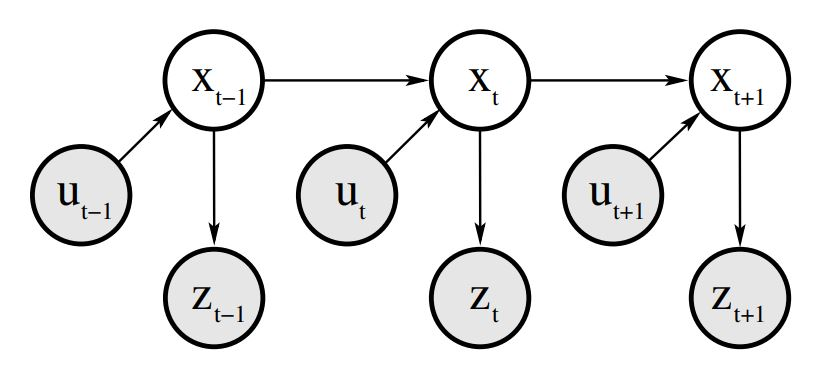
\includegraphics[width=0.75\textwidth]{markov.JPG}
    \caption{Lokaliseringsproblemet med Markovegenskapen är att bestämma $x_t$ givet $x_{t-1}$ och $u_t$. En bild på lokaliseringsproblemet som visualiserar Markovegenskapen för $x$, som kallas också för en Markovkedja \citep{ProbabilisticRobotics}.}
    \label{markov}
    \end{center}
\end{figure}

Robotens läge kan beräknas med Bayes filter som använder sig av rörelse- och landmärkesuppfattningssannolikheten \citep{ProbabilisticRobotics}. Bayes filter är en rekursiv algoritm som beräknar sannolikheten för robotens position baserat på robotens tidigare position, rörelseinformation och observerade landmärken. I Bayes filter algoritmen beräknas $bel(x_t)$, som är en sannolikhetsfördelning av robotens position i omgivningen.

\begin{algorithm}[H] \label{BFA}
    \SetAlgoLined
    \FuncSty{BayesFilter($bel(x_{t-1})$, $u_t$, $z_t$):} \\
    \ForAll{$x_t$}{
        $spådom$ = $\int P(x_t | x_{t-1}, u_t) bel(x_{t-1}) dx_{t-1}$ \\
        $bel(x_t)$ = $\eta P(z_t | x_t)$ $spådom$
    }
    \Return{$bel(x_t)$}
    \caption{Bayes Filter Algoritm}
\end{algorithm}

Bayes filters algoritmen fungerar så att för varje $x_t$ beräknas två kritiska steg, spådom och korrigering \citep{ProbabilisticRobotics}. Spådomsdelen i algoritmen är delen där vi beräknar integralen för två faktorer: sannolikheten att rörelseinformationen $u_t$ tar oss till $x_t$ och den gamla distributionen av positionen $bel(x_{t-1})$. Korrigeringsdelen är då man multiplicerar spådomsdelen med den sannolikhet att $z_t$ skulle observeras för varje möjliga $x_t$. I korrigeringsdelen används också en normering konstant $\eta$ för att normera sannolikheten. Bayes filter algoritmen är definierat ovan, se algoritmen \ref{BFA}. Utmaningen i algoritmen är att beräkna integralen i spådomsdelen. För att algoritmen skulle fungera i allmänhet, måste man begränsa robotens läge att vara en ändlig variabel så att integralen över spådomsdelen blir ändlig.

Med hjälp av Bayes regler, lagen om total sannolikhet för kontinuerliga variabler och Markovegenskapen kan det med matematisk induktion bevisas att Bayes filtern är korrekt, då man antar att $x_t$ har Markovegenskapen och att $bel(x_0)$ sannolikhetsfördelning är känd då $t = 0$. Med att sannolikhetsfunktionen är känd menar vi att roboten vet sin position vid början med full säkerhet eller så är $bel(x_0)$ en likformig sannolikhetsfördelning.
\begin{align}
bel(x_t) & = P(x_t | z_{1:t}, u_{1:t}) \tag{BF1}\label{BF1} \\
        & = \eta P(z_t | x_t, z_{1:t-1}, u_{1:t}) P(x_t | z_{1:t-1}, u_{1:t}) \tag{BF2}\label{BF2}\\
        & = \eta \underline{P(z_t | x_t)} P(x_t | z_{1:t-1}, u_{1:t}) \tag{BF3}\label{BF3}\\
        & = \eta P(z_t | x_t) \underline{\int P(x_t | x_{t-1}, z_{1:t-1}, u_{1:t}) P(x_{t-1} | z_{1:t-1}, u_{1:t}) dx_{t-1}} \tag{BF4}\label{BF4}\\
        & = \eta P(z_t | x_t) \int \underline{P(x_t | x_{t-1}, u_t)} P(x_{t-1} | z_{1:t-1}, u_{1:t}) dx_{t-1} \tag{BF5}\label{BF5}\\
        & = \eta P(z_t | x_t) \int P(x_t | x_{t-1}, u_t) P(x_{t-1} | z_{1:t-1}, \underline{u_{1:t-1}}) dx_{t-1} \tag{BF6}\label{BF6}\\
        & = \eta P(z_t | x_t) \int P(x_t | x_{t-1}, u_t) \underline{bel(x_{t-1})} dx_{t-1} \tag{BF7}\label{BF7}
\end{align}

Sannolikhetsfördelningen i Bayes filter är \ref{BF1}, det vill säga sannolikheten att roboten är vid $x_t$, som betecknas $bel(x_t)$, är samma som sannolikheten av $x_t$ givet $z_{1:t}$ och $u_{1:t}$. Med Bayes teorem kan detta skrivas om som i ekvation \ref{BF2}. För att få ekvationen \ref{BF3} använder vi Markovegenskapen för $x$, då kan betingade sannolikheten för $z_t$ skrivas som landmärkesuppfattningssannolikheten, $P(z_t|x_t)$. Med satsen om total sannolikhet för kontinuerliga variabler, som uttrycker sannolikheten för enskilda händelser till en betingade sannolikhet, kan formeln skrivas om till \ref{BF4} \citep[Kapitel~2.2]{ProbabilisticRobotics}. För att få ekvationen \ref{BF5} och \ref{BF6} använder vi Markovegenskapen för $x$, se Markovkedjan i figur \ref{markov}. Till slut får vi ekvationen \ref{BF7} som bevisar med induktion att algoritmen fungerar \citep{ProbabilisticRobotics}.

Bayes filter algoritmen baserar sig starkt på Markovegenskapen, det vill säga att det nuvarande läge är oberoende av tidigare data \citep{ProbabilisticRobotics}. I robotnavigering är det inte dock så lätt att anta detta, för det skulle betyda att allt runtomkring roboten är statiskt. Då man gör landmärkesuppfattningar kommer Bayes filter algoritmen att ge ett felaktigt estimat till exempel om en bil rör på sig då roboten navigerar. Bayes filter är basis för många andra lokaliseringsalgoritmer, som till exempel Kalman filter eller Markov lokalisation. 

I navigering är det svårt att begränsa robotens tillstånd så att integralen i Bayes filter blir en summa över spådomsdelen. Detta gäller endast om roboten navigerar i en begränsad omgivning. En begränsad omgivning kan vara till exempel en våning i en byggnad. För att åstadkomma robotar som navigerar autonomt i stora miljöer måste man approximera. Då möjligheterna av robotens läge är oändlig, till exempel utomhus, beräknar lokaliseringsalgoritmer ett approximativt värde för sannolikhetsfördelningen. Det är i beräkningen av approximativa värdet där olika lokaliseringsalgoritmer skiljer sig \citep{ProbabilisticRobotics}.

Genom att approximera sannolikhetsfördelningen lämnar man bort någon av egenskaperna som är viktigt för robotnavigering, såsom beräkningseffektivitet, noggrannhet i approximerande av robotens läge eller enkel implementering av algoritmen för robotar, för att till exempel förbättra någon annan av egenskaperna \citep{ProbabilisticRobotics}. Om man vill nå beräkningseffektivitet då man approximerar så avstår man till exempel i noggrannhet av robotens läge.

Lokaliseringsproblemet kan delas i global och lokal lokalisering \citep{982903, globalsubmaps}. Med global lokalisering har roboten ingen vetskap om sin position vid början av navigeringen. I lokal lokalisering har roboten en ungefärlig eller exakt vetskap om sin plats vid början av navigeringen som den fått som indata. Då man använder sig av globala lokaliseringsmetoder är sannolikheten att roboten är vid $bel(x_0)$ en likformig sannolikhetsfördelning över alla lägen i stokastiska variabeln $X$ och i lokala lokaliseringsmetoder är det till exempel $bel(x_0) = 1$ eller en normalfördelning runt läget $x_0$ \citep{ProbabilisticRobotics}. Lokala lokaliseringsmetoder strävar för att korrigera fel som uppstår av robotens rörelse. Med globala lokaliseringsmetoder kan roboten klara av verkliga misstag då den estimerar sin position i omgivningen, till exempel roboten kan klara av en situation där den kidnappas och förs till en annan plats.

\section{Kartläggning av omgivningen} \label{kartlaggning}

Med kartläggning av omgivningen menar vi att en robot använder data den har tillgång till för att kartlägga sin omgivning. Detta kan vara till exempel rörelseinformation eller sensorinformation samt kombinationer av dessa \citep{ProbabilisticRobotics}. I lokal lokalisering, där man vet robotens läge och har åtkomst till rörelseinformation, är kartläggning lättare att göra än då robotens position i början är okänd. För att konstruera en karta så måste man ta i beaktande störningar som uppstår av rörelse- och sensorinformation.

En karta om miljön kan representeras i två (2D) eller tre (3D) dimensioner \citep{geospatial}. Att konstruera en 3D-representation av omgivningen kräver det mer beräkningskapacitet än att konstruera en 2D-karta \citep{ProbabilisticRobotics}. För robotar som navigerar på stadig grund är oftast en 2D-representation tillräckligt, men för drönaren behöver man kartlägga i 3D. 

För att konstruera 3D-kartor behöver man uppskatta djup. Metoder för att uppskatta djup med datorseende är till exempel beräkning av binokulära skillnaden eller rörelseparallax \citep{suomimainittu}. Rörelseparallax betyder att objekt rör på sig snabbare i synfältet då de är närmare observatören och långsammare då de är långt borta. Detta gäller också om observatören rör på sig och objektet står stilla \citep{suomimainittu, parallax}. För att räkna binokulära skillnaden för observerade kännetecken behöver man två kameror som är riktade parallellt i samma linje så att deras synfält överlappar, kamerornas distans från varandra är känd och från båda kamerornas bilder utdras samma kännetecken. Från skillnaden mellan kännetecknets horisontala position i båda av kamerornas bilder går det att estimera djup. Med en monokulär kamera kan man uppskatta djup i bilder baserat på rörelseparallax. För detta behöver man veta distansen till ett objekt då navigeringen börjar. Som indata för beräkningen får man bilder och rörelseinformation av roboten. Rörelseinformationen i robotar på stadig grund kan man få till exempel från en hastighetsmätare som är inbyggt i roboten.

\cite{suomimainittu} undersökte djupuppskattning med rörelseparallax. Genom att räkna binokulära skillnaden från stereokameror märkte de att stereokameror fungerar bättre då objekten är nära medan monokulära kameror kan uppfatta mer precis distans på långt håll \citep{suomimainittu}. Med stereokamera kan djup estimeras bra upp till cirka 10 meters avstånd och vid 20 meters avstånd så är estimeringarna oanvändbara. Vid 20 meters avstånd måste man växla över till att använda monokulära kameran. \cite{suomimainittu} skriver att forskning för att skaffa rörelseinformation från bilderna är viktigt, på grund av att rörelseinformation behövs för att lokalisera roboten i omgivningen och kartlägga omgivningen. Genom att uppskatta rörelseinformation från bilder kan man avlägsna hastighetsmätare som drönare inte har tillgång till. Detta ger möjlighet att estimera djup för drönare.

Kartor kan sparas i olika format, såsom datorstödd konstruktion (CAD, Computer-Aided Design), beläggningskarta (Occupancy Grid Map) eller en enkel graf om landmärken och deras sammankopplingar \citep{982903}. En datorstödd konstruktion av miljön kan vara en mycket detaljerad representation av omgivningen. En beläggningskarta är en 2D eller 3D-modell av omgivningen som är sparat i ett rutsystem där rutor som är upptagna är någon objekt i miljön, oftast har dessa rutorna sparat i sig en sannolikhet att där finns någon objekt i vägen \citep{6095058, 982903}. Kartan kan vara färdigt sparad för en drönare eller så kan miljön kartläggas med hjälp av bilderna från sensorerna då den flyger \citep{geospatial}. Med 3D volymetriska sensorer kan man konstruera en 3D modell och spara denna information i en Octree-struktur. Med strukturen kan data om miljön packas i mindre format utan att tappa möjligheten att uppdatera informationen vid behov. En annan metod som tas upp är med stereovisionsalgoritmer göra en djupkarta och behandla data till plana ytor som minskar på missvisning som uppstår med användning av stereovision algoritmer när man bygger upp djupkartan. 

Oftast har robotar inte en färdig karta som de kan använda för att planera sin rutt eller att navigera \citep{ProbabilisticRobotics}. För att åstadkomma autonoma robotar måste de själv kunna kartlägga sin omgivning. Kartläggning för robotar är ett problem som är svårt utan lokalisering och lokaliseringsproblemet är svårt att lösa utan att man kartlägger, därför är det nyttigt att lösa båda problem samtidigt. 

\chapter{Samtidig lokalisering och kartläggning} \label{slamchap}

Samtidig lokalisering och kartläggning (SLAM) är ett av de grundläggande problem inom robotnavigering \citep{realslamproblem}. SLAM-problemet definieras så att en robot som inte har tidigare information om sin plats eller omgivning skall samtidigt bygga en karta av omgivningen och lokaliserar sig själv relativt till kartan som den bygger, till exempel med hjälp av datorseende och att identifiera landmärken. Med att beräkna robotens läge menar vi beräkningen av $P(x_t, m|z_{1:t}, u_{1:t})$, det vill säga, sannolikheten att roboten befinner sig vid $x_t$ och kartan $m$ givet alla landmärkesuppfattningar $z_{1:t}$ och rörelseinformation $u_{1:t}$. 

Det finns två varianter av SLAM-problemet: Fullständig SLAM och Online SLAM \citep{ProbabilisticRobotics}. Skillnaden med dessa två är hur man beräknar betingade sannolikheten för $x_t$ och $m$. I Fullständig SLAM beräknas betingade sannolikheten för hela robotens positionskedja $x_{0:t}$, det vill säga $P(x_{0:t}, m | z_{1:t}, u_{1:t})$, medan i Online SLAM använder man bara senaste läge $x_{t}$ och kartan $m$, då är formeln $P(x_t, m | z_{1:t}, u_{1:t})$, alltså döljer tidigare rörelse- och landmärkesinformation för att estimera den nya positionen av roboten. Några lösningar för SLAM som baserar sig på sannolikhetsberäkning är Extended Kalman Filter (EKF-SLAM), som är en Online SLAM-lösning, och FastSLAM, som är en Fullständig SLAM-lösning \citep{realslamproblem, ProbabilisticRobotics}. 

\begin{figure}[ht]
    %\begin{figure}[tbh] t= top, b = bottom, h=here
    \begin{center}
    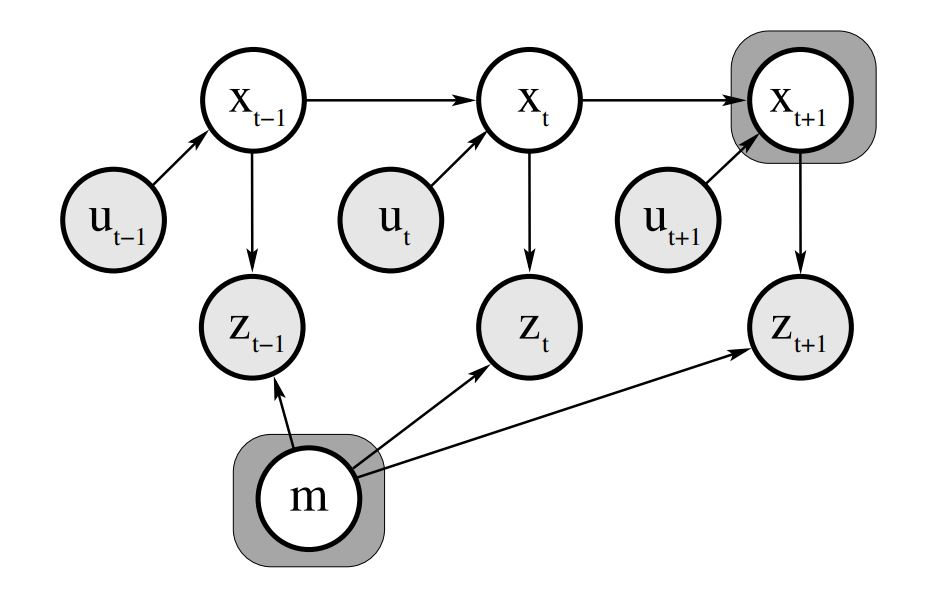
\includegraphics[width=0.75\textwidth]{online-slam.JPG}
    \caption{Bild på Online SLAM-problemet där man beräknar sannolikheten av robotens position och bygger kartan från sensorinformation $z$ och rörelseinformation $u$ \citep{ProbabilisticRobotics}.}
    \label{slam-problemet}
    \end{center}
\end{figure}

SLAM-problemet har delproblem som måste lösas för att åstadkomma autonoma robotar \citep{slamproblem}. Ett stort problem i flesta visionsbaserade SLAM-lösningar är dataföreningsproblemet. Detta betyder att man identifierar två olika landmärken som en och samma. Problem kan uppstå redan vid korta rörelsen av robotar eller då en robot har navigerat och kommer till en plats som den redan har varit i vid, detta kallas för loopstängning (Loop Closure). Med att förena landmärken fel så uppkommer det missvisningar då man estimerar positionen av roboten.

Positionen av roboten i omgivningen och landmärkens position i kartan kan också beräknas med att räkna distansen till landmärken och bevara en matris med landmärkens sannolikhetsposition i omgivningen och landmärkes förhållande till varandra, alltså en korrelationsmatris \citep{realslamproblem, ProbabilisticRobotics}. Genom att bevara en korrelationsmatris så har man den fördelen att när man lokaliserar en robot går det med stor sannolikhet att uppdatera sannolikhetsfördelningen för alla landmärkes positioner. Nackdelen med denna metod är att då man observerat stora mängder av landmärken så kommer beräkningsbehovet att växa kvadratiskt enligt antalet observerade landmärken. 

Visuell kartläggning och lokalisering kan delas i tre kategorier baserat på data som man har i början av navigeringen. Kategorierna är kartlösa (mapless), kartbaserade (map-based) och kartbyggande (map-building) system \citep{geospatial}. 

\section{Kartlösa system}

Kartlösa situationen är oftast den realistiska system då man navigerar \citep{ProbabilisticRobotics}. I system utan karta navigerar drönare bara med hjälp av att observera tydliga egenskaper i miljön \citep{982903}. Dessa kan vara till exempel väggar, dörrar, möbler eller andra landmärken. Metoder för navigering i kartlösa system, som diskuteras i avhandlingen, är optiskt flöde (Optical flow) och spårning av egenskaper (Feature tracking). 

\subsection{Optiskt flöde}

Optiskt flöde hänvisar till uppfattad relativ rörelse i sekventiella bilder mellan observatören och till exempel någon fästpunkt i miljön \citep{opticalflowuav}. Rörelse uppstår i sekventiella bilder till exempel då man vänder kameran eller om något rör på sig då kameran är stilla. En flödesvektor beskriver till exempel hastigheten av en robot eller ett objekt som rör på sig. Flödesvektorn beräknas från skillnaden var objektet befinner sig i bilderna.

För att demonstrera ett exempel hur optiskt flöde kan användas för robotnavigering har \cite{341094} använt optiskt flöde i en robot för att få robotar att imitera bin \citep{341094}. De placerade två kameror som är parallellt riktade ifrån varandra på varsin sida av en robot och beräknade flödesvektorer från bilderna ur båda kameror då roboten rör på sig. Om flödesvektorernas beräknade längd var samma på båda sidorna så far roboten rakt framåt. I situationen där flödesvektorerna är av olik längd vänder roboten mot den sida där vektorn är kortare. Genom att använda optiskt flöde för navigering behöver man inte uppskatta djup. Denna navigeringsmetod fungerar dåligt i strukturlösa miljöer där det inte finns några fästpunkter eller landmärken som kan användas för att beräkna flödesvektorerna.

Metoden som \cite{341094} använde tog bara i beaktande horisontala flödesvektorer och demonstrerade att optiskt flöde kan användas i robotnavigering på stadig grund. Sedan detta har användning av optiska flödesmetoder använts i drönare \citep{6564752}. Nuförtiden används optiskt flöde av drönaren för att uppskatta avstånd mellan drönaren och objekt, hålla sin höjd, undvika hinder, beräkna hastighet och landa på en plattform som rör på sig.

\subsection{Spårning av egenskaper}

Spårning av egenskaper (Feature tracking) används för att skaffa information om objekt, såsom linjer, hörn och olika landmärken som är invarianta för rörelse, med hjälp av kameror och bildbearbetningsalgoritmer \citep{geospatial}. Med hjälp av dessa landmärken och deras relativa rörelse i sekventiella bilder kan man bestämma robotens position och bygga en karta. Då drönare navigerar i omgivningen, så kommer den troligtvis att se samma landmärken från olika perspektiv. Detta hjälper drönaren att beräkna en bättre sannolikhet för sin position i omgivningen samt uppdatera landmärkenas position i kartan. Traditionella SLAM-lösningar, såsom EKF-SLAM och FastSLAM faller under denna kategori \citep{voslamlatif}. Dessa SLAM-lösningar fungerar inte då det finns mycket landmärken i kartan för till exempel med EKF-SLAM är problemet beräkningsbehovet som växer kvadratiskt av antalet landmärken.

För att drönaren har begränsad batterikapacitet och bärkraft har \cite{voslam} föreslagit användning av VOSLAM (Visual Odometry SLAM). VOSLAM kan kartlägga omgivningen och lokalisera observatören då det finns upp till tusentals landmärken i kartan med hjälp av en stereokamera och en krets som konsumerar tio gånger mindre energi än en Intel i7 3770K-processor \citep{voslam}. Deras VOSLAM algoritm implementeras i en FPGA-krets (Field-Programmable Gate Array) vars logik är omprogrammerbar. Kretsen använder färre energi än vanliga processorer och kan beräkna parallellt. VOSLAM, med speciell hårdvara, klarar av upp till 30 000 landmärken i kartan, jämfört med EKF-SLAM, som klarar av kring tusen landmärken för att fungera i realtid \citep{ProbabilisticRobotics, voslam}.

VOSLAM-lösningen fungerar så att den extraherar landmärken från bilder med bildbearbetningsalgoritmen SIFT \citep{voslam}. Med hjälp av att beräkna binokulära skillnaden från bilder för att uppskatta djup, som diskuterades i kapitel~\ref{kartlaggning}, konstruerar de en 3D-representation av dessa landmärken. Med FPGA-kretsen beräknas vektorvinklarna för varje landmärke. Då roboten navigerar kan de matcha observerade landmärken med de som de har i kartan för att lokalisera drönaren. 

Enligt \cite{voslam} estimerar VOSLAM positionen av drönaren, hantera loopstängning och är en energieffektiv lösning för SLAM-problemet \citep{voslam}. Något som deras lösning inte tar i beaktande är SIFT-algoritmens tidskrav, det vill säga växande beräkningsbehovet. \cite{voslamlatif} demonstrerade att VOSLAM fungerar för drönare också då SIFT-algoritmens tidkrav tas i beaktande \citep{voslamlatif}. De dela upp processen i två delar: Byggande av 3D-representationen ur omgivningen görs med SIFT i en egen processor, och uppdatering av kartan, matcha observerade landmärken med kartan, lokalisering av drönaren hanterades i FPGA-kretsen \citep{voslamlatif}.

\section{Kartbaserade system}

I kartbaserade system har drönaren en färdig vetskap om miljön som kan vara i form av geometriska modeller, beläggningskarta eller förhållande mellan landmärken \citep{982903}. Idén är att då roboten navigerar så prövar den hitta landmärken från bilder som är lika med de landmärken som roboten vet om. När den observerat landmärken och förenat observationerna med kartan som den har, beräknas sannolikheten av robotens position i miljön. Med kartbaserad navigering kan en drönare planera sin rutt i förhand och beräkna omvägar under navigeringen då det behövs \citep{geospatial}. 

Kartbaserad lokalisering med datorseende kan delas upp i fyra steg \citep{982903}:

\begin{itemize}
    \item skaffa sensorinformation
    \item upptäcka landmärken från informationen med bildbearbetning
    \item matcha observationerna med landmärken i kartan
    \item estimera positionen av roboten
\end{itemize}

Det svåraste steget av dessa är att matcha observerade landmärken korrekt med de landmärken som finns i kartan. Roboten kan inte med full säkerhet veta sin position och då är det svårt att matcha landmärken korrekt med de landmärken som finns i kartan \citep{982903}.

Då kartan finns kan man fokusera på lokalisering av roboten \citep{982903}. I global lokalisering måste man lita på att man kan förena observationerna med informationen man har och ta i beaktande osäkerheten med att observationerna kan matcha flera av landmärkena man vet om. Globala lokaliseringsproblemet, där roboten inte har en aning om var den är på kartan vid början, kan till exempel lösas med Monte Carlo lokalisation eller Markov lokalisation. Båda av algoritmerna är en variant av Bayes filter som presenterades i kapitel~\ref{lokalisering} \citep{ProbabilisticRobotics}. 

I Monte Carlo lokalisation antar en robot med lika sannolikhet sin position i kartan vid början av navigeringen \citep{montecarlo}. Då man approximerar sannolikheten av robotens position väljer man slumpmässigt kandidater för platser där roboten möjligen skulle befinna sig med den rörelseorder som den tar. Efter det rör roboten på sig och observerar landmärken. Sedan identifieras de observerade landmärken ur de som finns i kartan. På basis av de landmärken som den har observerat och identifierat med kartan kan roboten estimera vilken av dessa slumpmässiga positionsval var den bästa. 

Markov lokalisationsalgoritmen klarar också av globala lokaliseringsproblemet då man har en karta \citep{ProbabilisticRobotics}. Istället för att bara anta en sannolikhet för robotens position i kartan så uppehåller den en sannolikhetsfördelning över hela kartan. Mer specifikt, då roboten börjar navigera är sannolikhetsfördelningen enhetlig. Efter att roboten har rört på sig observerar den landmärken och matchar dessa landmärken med de som är i kartan. För varje match den hittar i kartan ökar sannolikheten att roboten befinner sig nära dessa landmärken. När den rör på sig vidare så kommer den troligtvis att observera mera landmärken och på basis av rörelseinformationen och observerade landmärken kan den vid något skede vara ganska säker av sin position i kartan.

I lokal lokalisering där roboten har en vetskap om sin position i början av navigeringen behöver algoritmen hålla koll på rörelsen som roboten utför. På basis av rörelseinformationen förbättras uppskattningen av robotens position \citep{montecarlo,ProbabilisticRobotics}. Då roboten rör på sig minskar sannolikheten av robotens position på basis om hur algoritmen tar i beaktande felmarginal i rörelsen. Då osäkerheten av sin egen position är för stor så använder den observerade landmärken och matchar dessa med kartan för att öka på sannolikheten av sin position. 

\section{Kartbyggande system}

Kartbyggande system används då det är svårt att navigera med en existerande karta om omgivningen eller om kartan inte finns. Exempel av sådana områden är till exempel katastrofområden \citep{geospatial}. Fördelar med att bygga en karta i 3D och använda denna för lokalisering är att det uppkommer mindre missvisningar då roboten lokaliserar sig själv för det finns mera detalj. I 2D-kartor då en robot navigerar i en korridor och kommer till slutet av korridoren kan det vara svårt för roboten att veta i vilken ända den är om korridoren är symmetrisk. Med 3D så finns det mera data att använda för att lokalisera. Detta betyder dock att man även behöver mera beräkningskapacitet. Kartbyggande systems bildbearbetning kan delas i tre kategorier, som är indirekta, direkta och hybrida metoder. Den sistnämnde sammanslår indirekta och direkta metoder \citep{geospatial}. I denna avhandling diskuteras indirekta och direkta metoder.

\subsection{Indirekta metoder}

I bildbearbetning som använder indirekta metoder tar man kännetecken ur bilden som är invarianta för rotation, synvinkeländringar och rörelseoskärpa, dessa ges som indata som sedan kan användas för rörelseuppfattning och lokalisering \citep{geospatial}. 

Ett sätt att konstruera en karta är att beakta robotens rörelse och synvinkel \citep{globalsubmaps}. \cite{mapbuildingsift} har gjort dessa samt använt indirekta metoder i sin artikel \citetitle{mapbuildingsift} för att bygga en 3D-karta \citep{mapbuildingsift}. Från stereokamerornas bilder, utjämnar de bilderna så att de har mindre detalj i sig och använder SIFT för att extrahera egenskaper ur bilderna. Med denna metod har de kunnat konstruera en 3D-karta av omgivningen baserat på landmärken utan att spara korrelationsmatris mellan landmärken som minskar på behov av beräkning då man lokaliserar roboten. Denna metod för att konstruera kartor och lokalisera roboten har ändå problem då det kommer till loopstängning och uppdatering av kartan \citep{globalsubmaps}. Med att använda samma bildbearbetningsmetoder och kartlägga delar av områden och senare bygga en stor global karta fick forskarna loopstängningen och kart-uppdateringen minskad. Globala kartan uppbyggdes genom att identifiera identiska landmärken från dessa små kartor och från dessa fogades ihop kartor som var bredvid varandra till en stor karta. Indirekta metoder fungerar dåligt då det finns få egenskaper att extrahera ur bilder, såsom i strukturlösa miljön \citep{geospatial}.

\subsection{Direkta metoder}

Direkta metoder fungerar bra i miljön där det finns lite detalj att extrahera ur bilder \citep{Engel2014LSDSLAMLD}. Jämfört med indirekta metoder där man prövar hitta många landmärken ur bilderna så använder direkta metoder hela bilden för att hitta geometriska egenskaper. Med hjälp av dessa kan man konstruera en detaljerad karta \citep{geospatial}. Då man konstruerar en mycket detaljerad karta går det också att använda kartan för något annat än navigering, som till exempel att få information från katastrofområden. Att kartlägga i detalj används bara i speciella fall för drönare, på grund av att det kräver mycket beräkningskapacitet och förbrukar mycket energi.

\chapter{Sammanfattning}

Samtidig lokalisering och kartläggning i dynamiska miljön är ett centralt problem som måste lösas för att drönare skulle kunna navigera autonomiskt. Oftast är robotens omgivning oändlig och då man beräknar positionen av roboten måste man approximera. Då man approximerar sannolikheten av robotens position är den sällan fullständigt medveten om sin position. 

För att verkligen ha autonoma drönaren, som kan använda sig av visionsbaserad navigering, måste man kunna kombinera effektiva bildbearbetningsalgoritmer, lokaliseringsalgoritmer och kartläggningsalgoritmer så att dessa algoritmer skulle fungera samtidigt, i realtid samt ge bra uppskattningar av drönarens läge. 

En drönare har begränsningar då det kommer till beräkningsbehov på grund av att kommersiella drönare byggs mindre än förr och har begränsad batterikapacitet. Drönare har inte tillgång till samma rörelseinformation som robotar på stadig grund som oftast har inbyggda tröghets- och hastighetsmätare i sig. Därför är det viktigt att det finns forskning inom beräkning av rörelseinformationen från kamerabilder. 

I denna avhandling gavs en ytlig översikt om SLAM-problemet och vad är basis för de SLAM-lösningar som finns idag. Även om de existerande lösningarna är fungerande finns det ännu ett antal utmaningar som borde bemötas. Utmaningarna är att konstruera pålitliga algoritmer inom visionsbaserad navigering som kan behandla olika scenario, till exempel kartläggning och lokalisering i dynamiska miljöer. Utmaningar som inte diskuterades i avhandlingen är ruttplanering och hur drönaren undviker hinder under navigeringen, vilka är också viktiga för att åstadkomma autonoma drönaren.

